%!TEX root = ../Base.tex

\chapter{Speaker diarisation}\label{ch:chap5}

Se conoce como \SD~ al problema de segmentación automática de audio a partir de la identificación de las diferentes personas que participan en una grabación. Esto se realiza generalmente identificando los segmentos que son más \textit{homogéneos} y a partir de estos, identificar el número de personas que hablan en la grabación.

Se considera que cada persona posee ciertas características propias que la diferencian de los demás. Por ejemplo, tanto la tesitura como el timbre son rasgos que varían de persona a persona.

La idea básica cuando se busca abordar este problema es el de poder segmentar la señal de audio de acuerdo a los cambios que ocurren en ésta. Es decir, detectar por ejemplo las variaciones en la voz (que usualmente implican que alguien más está hablando) y luego, con todos los segmentos obtenidos, tratar de agruparlos según características similares; pues una misma persona tiene características propias en su voz. 

\section{Aplicaciones de \sd}

Por la misma naturaleza del algoritmo, cuando se realiza \sd, lo que se trata de inferir es cuántas personas hablan, y cuándo habla cada una de ellas; es decir, se identifica a un grupo $n$ de personas, pero no se dice nada acerca de ellos o su identidad. 

Por el mismo planteamiento del problema, las etiquetas asignadas a cada persona identificada en la grabación puede cambiar, pues no hay nada que nos permita asociar de manera no arbitraria una etiqueta a una persona en especifico. Es decir, el orden en que se asignan las etiquetas puede cambiar, aunque la segmentación obtenida sea en esencia la misma.

La segmentación y agrupación de voz, es una parte importante de la transcripción de voz, así como también del reconocimiento de voz e identificación de personas que hablan. 

Es de gran ayuda para la tarea de reconocimiento de voz, puesto que éste se basa en identificar palabras completas; por lo que al lograr segmentar una señal de audio de acuerdo a las personas que hablan, se tendrá entonces muy seguramente una buena segmentación tanto de palabras como oraciones completas.

En cuanto a la identificación de personas y alguna otra modelación acústica que se quiera realizar; es importante que los modelos que se entrenan usen segmentos de audio homogéneos (en este caso, que se tenga la certeza que corresponden a la misma persona), para que en realidad se esté modelando la voz de la persona, y no algo diferente a ella.

Como último ejemplo, la transcripción automática de voz, es el proceso en el que además de lograr identificar cuándo habla cada persona, se identifica de quién se trata realmente esta persona, y qué es lo que está diciendo. Ésto sirve por ejemplo, cuando se tiene una gran cantidad de grabaciones de audio; y se desea etiquetar de qué se habla en cada una de estas grabaciones. 

\section{Procesamiento de señal}

Antes de abordar de lleno el problema de \sd, se tiene que realizar cierto tratamiento a la señal de audio con la que se trabajará. 

Es decir, a partir de la señal de entrada (que se considerará es digital) se tratarán de obtener vectores de características cada cierto tiempo, que representen de forma adecuada los rasgos que nos interesan distinguir.

Una vez que se tienen estos vectores, se les aplica un algoritmo de aglomeración para entonces obtener un conjunto de etiquetas que se podrían considerar como posibles estados o palabras de diccionario referentes a la señal de audio.

El proceso en detalle se especifica a continuación: 
\subsection{Esquema general del sistema}

--Insertar dibujo y explicarlo--.

\subsection{Pre-procesamiento de señal de audio}

Se considera que se tiene una señal digital de voz, y que a partir de ésta se identificarán a las diferentes personas que hablan durante la grabación.

\begin{figure}[bth]
  \myfloatalign
  {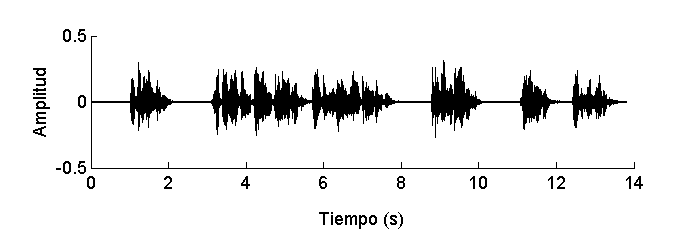
\includegraphics[width=0.9\linewidth]{gfx/chap5/signal-orig}} \quad
  \caption{Señal original de audio.}
  \label{fig:sign_orig}
\end{figure}

El primer paso en el procesamiento de la señal, es tanto la detección como eliminación de silencios; pues éstos realmente no nos interesan para la modelación del sistema.

\graffito{Nota: Tanto en ancho de la ventana, como el umbral para definir si será silencio se pueden ajustar dependiendo del tipo de señal.}

Para realizar entonces la detección de los silencios, en esta primer etapa y como un primer intento para la eliminación de silencios, se hace una detección básica de qué partes de la señal son mayormente silencios.

Para ésto, se utiliza una ventana móvil que se irá recorriendo a lo largo señal, y que irá calculando el total de energía de la señal dentro de la ventana. Se considerará entonces silencio aquellas partes de la señal cuyo total de energía esté debajo de un umbral específico.

A partir de esta ventana se obtienen entonces las regiones que pertenecen tanto al silencio, como a la señal que realmente se desea modelar.

\begin{figure}[bth]
  \myfloatalign
  \subfloat[Señal original con silencio identificado.]
  {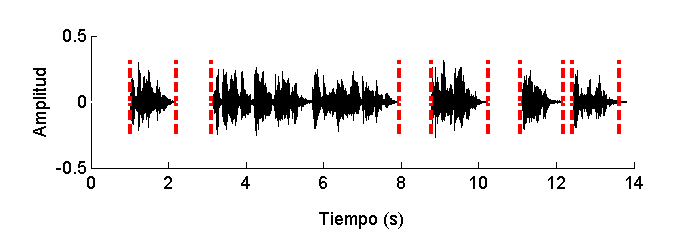
\includegraphics[width=0.9\linewidth]{gfx/chap5/signal-silence}} \quad
  
  \subfloat[Señal procesada y recortada.]
  {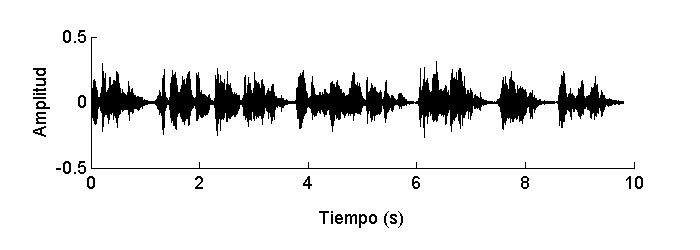
\includegraphics[width=0.9\linewidth]{gfx/chap5/signal-trunc}} \quad
  
  \caption{Identificación y eliminación de silencio en señal.}
  \label{fig:sig_silence}
\end{figure}

Como se observa en la \autoref{fig:sig_silence} basta entonces con eliminar los segmentos que con baja energía y reagrupar la señal restante.

Con esto, se obtiene una señal en general más pequeña, y que se podría  considerar sólo contiene realmente los datos que se desea modelar.

\subsection{Obtención de características acústicas}

Una vez que se tiene la señal ya sin silencios, se trata de buscar características propias de la señal de audio que nos permitan identificar de buena forma los cambios de voz a través de la señal.

Tanto la extracción como selección de la mejor representación paramétrica de la señal de audio es una importante tarea en el diseño de cualquier sistema relacionado al reconocimiento o procesamiento de señales de audio. 

Para la tarea de \sd, se usarán los Coeficientes Cepstrales de Frecuencia Mel  (\MFCC), que son ampliamente utilizados por ejemplo en \textit{speech recognition} entre otros procesos relacionados al procesamiento de voz; cuyo objetivo es comprimr la señal de audio eliminando la información que no es útil para análisis fonético.

Cabe mencionar, que originalmente los \MFCC~ fueron diseñados para la tarea específica de reconocimiento de voz [referencia ICASSP 82], por lo que al momento de diseñarlos se trataba principalmente de que una misma palabra  fuera parametrizada de la misma manera sin importar quién fuera quien la pronunciara. 

Ésto va en contra del proceso requerido en \sd, puesto que se desea identificar a las diferentes personas que hablan, sin dar tanta importancia a qué es lo que están diciendo; por lo que la tarea de segmentación de señales de audio se vuelve un poco más complicada.

Para calcular los \MFCC, se usa la Escala de Frecuencia Mel, que está espaciada de forma lineal en frecuencias bajas, mientras que aumenta su separación de forma logarítmica para frecuencias más altas. Este cambio de separación se realiza comúnmente a partir de los $1000Hz$. 

A partir de esta escala, se diseña un banco de filtros triangulares que después se usará (Ver \autoref{fig:sign_melfb}); y esto corresponde de forma similar a la que el oído (la cóclea) captura las características importantes del habla. 

\begin{figure}[bth]
  \myfloatalign
  {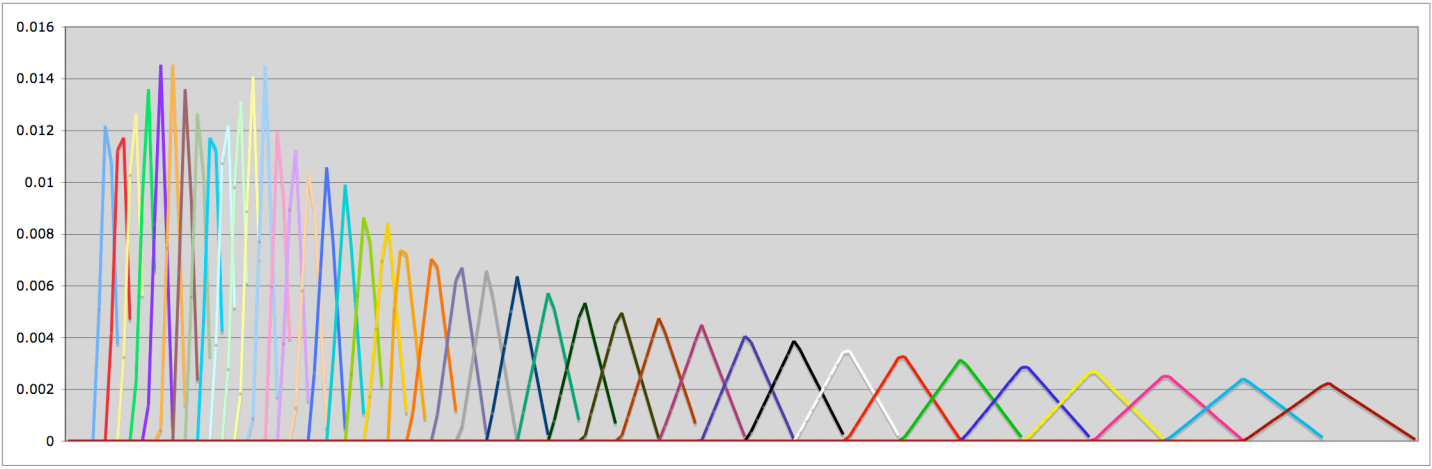
\includegraphics[width=0.9\linewidth]{gfx/chap5/melfb}} \quad
  \caption{Banco de filtros triangulares en frecuencia Mel.}
  \label{fig:sign_melfb}
\end{figure}

Puesto que el banco de filtros de Mel trabajan en la frecuencia; a la señal de audio se le aplica la transformada de Fourier, y entonces a ésta es a quien se le aplica el banco de filtros.

Sea pues \autoref{fig:sign_orig} una señal 